\section{Overview of the MicroBooNE Experiment}
\label{Chapter:2}
The Micro Booster Neutrino Experiment (MicroBooNE) features the first large-scale LArTPC exposed to both the Booster Neutrino Beam (BNB) and Neutrinos at the Main Injector (NuMI) beamlines at Fermilab. The LArTPC is located at $470$ m on-axis from the BNB target and $679$ m and $3^{\circ}$ off-axis from the NuMI target. MicroBooNE's primary goal is to provide further insight into the low energy anomalies observed by MiniBooNE, mentioned in Chapter \ref{Chapter:1}. Beyond that, it aims to measure neutrino-LAr cross-sections and further develop the LArTPC technology. It took data from 2015 to 2021 and produced dozens of physics results; dozens more are in the works. 
In this chapter, I will describe MicroBooNE's LArTPC and light collection system, the NuMI beamline, and the data acquisition and processing. I will not go into details about the BNB beamline as it escapes the scope of this work.

\section{The Detector}

In this section, I will briefly describe the two main components of the MicroBooNE detector: the LArTPC and the light collection system.
\subsection{Time Projection Projection Chamber}
As extensively explained in Chapter \ref{Chapter:1}, LArTPCs are very powerful detectors for neutrino physics. They allow tracking reconstruction with precision calorimetric information and event displays that resemble bubble-chamber ones. MicroBooNE's LArTPC is $10.4$ m long along the BNB beam direction (z-coordinate), $2.56$ m wide in the drift direction (x-coordinate), and $2.33$ m tall (y-coordinate). Referred to as the ``active volume", this corresponds to $87$ tons of liquid argon 

The MicroBooNE LArTPC has $3$ planes of wires, $2$ of which are called ``induction planes" and produce a bipolar signal when electrons pass through them. One induction wire plane (the U plane) has the wire oriented on $+60^{\circ}$ angle with the vertical, and the other (the V plane) $-60^{\circ}$ angle with the vertical. The third is the collection plane (Y plane), oriented vertically, which will collect the electrons, producing a unipolar signal \cite{microboone_electronics}. In figure \ref{uboone_digital_signal} you can see each plane's signal shape. The $3$ wire planes together form a structure called the anode plane assembly (APA). 

\begin{figure}[h!]
	\begin{center}
		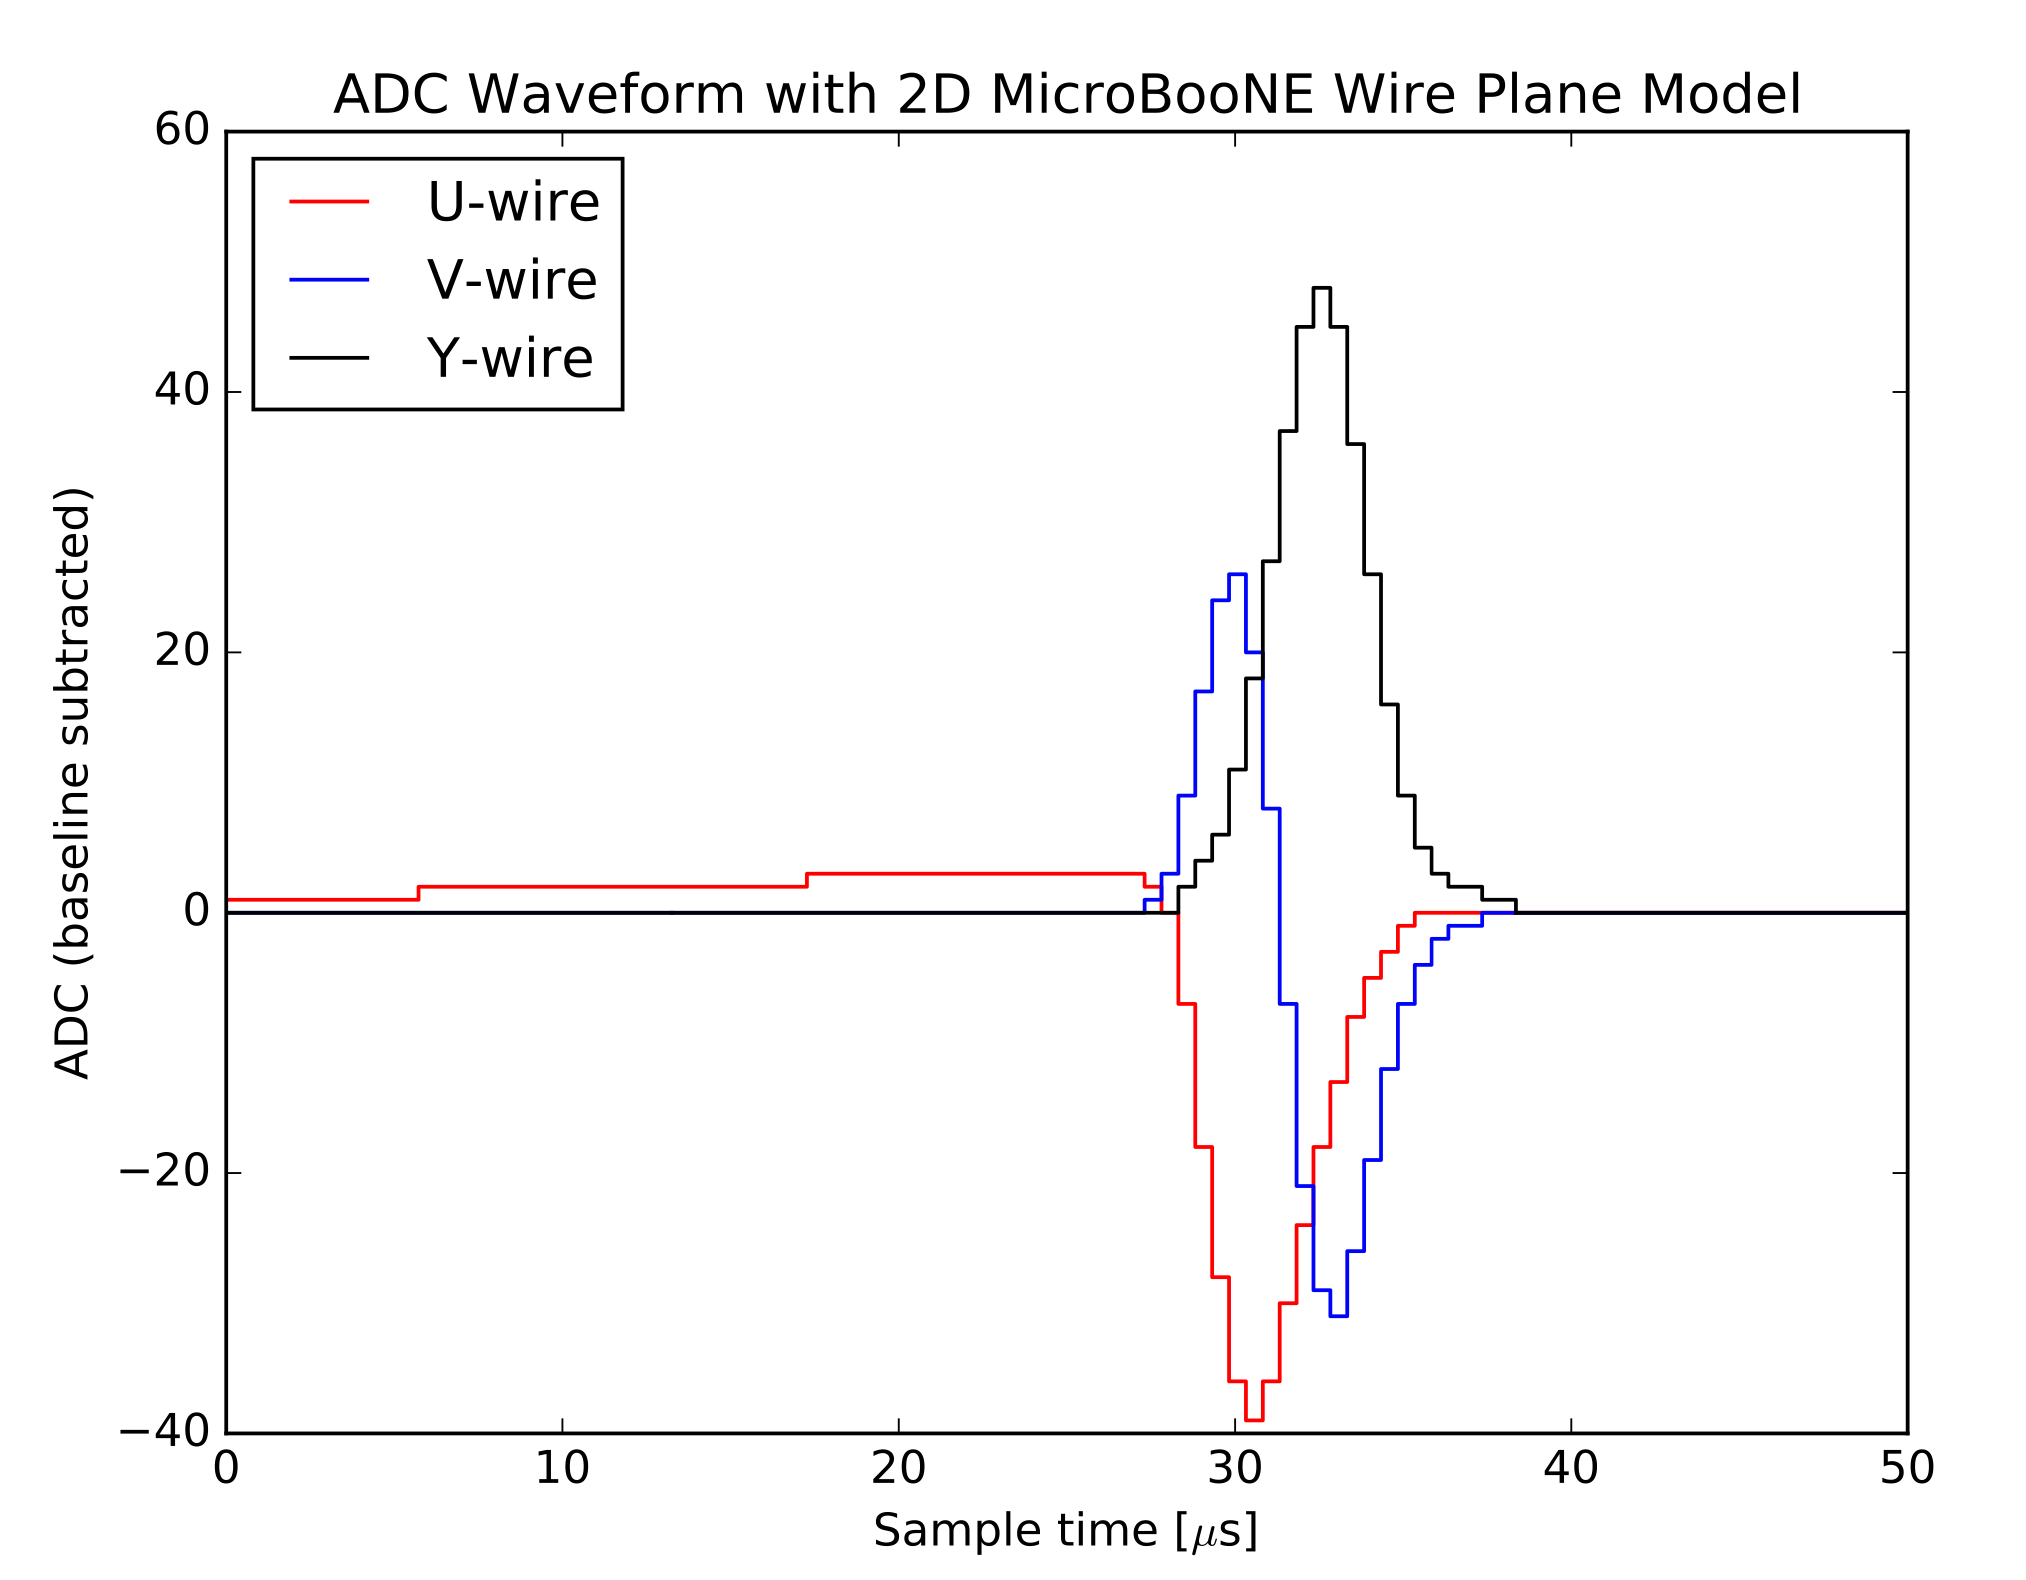
\includegraphics[scale=0.25]{Figures/uboone_dig_signal.png}
		\caption[MicroBooNE's wire planes digital signal]{{\textbf{MicroBooNE's wire planes digital signal}}  \\ The U (V) plane corresponds to the induction wires at $+60$ ($-60$), and induction signals are bipolar in shape. The Y plane corresponds to the vertically-oriented collection wires, whose signals are unipolar in shape.”
        \cite{microboone_electronics}}
		\label{uboone_digital_signal}	
	\end{center}
\end{figure}

A picture of MicroBooNE's assembled LArTPC can be seen in figure \ref{uboone_lartpc} All three planes have a wire spacing of $3$ mm. The cathode of the LArTPC is at $-70$ kV, and the middle induction plane in the APA is at ground, creating an electric field along the drift direction of $273$ V/cm. At total, MicroBooNE's LArTPC has $8,256$ wires \cite{microboone_design}. 

\begin{figure}[h!]
	\begin{center}
		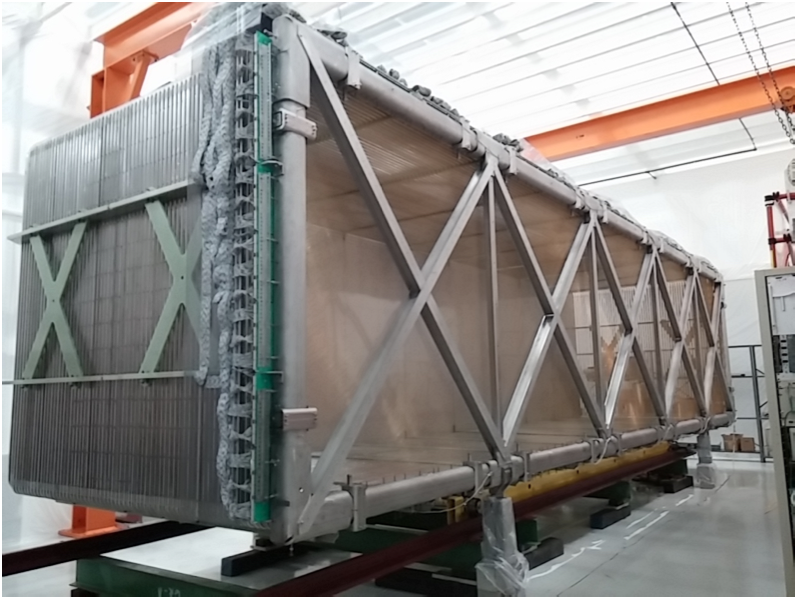
\includegraphics[scale=0.6]{Figures/uboone_LArTPC.png}
		\caption[MicroBooNE's Liquid Argon Time Projection Chamber]{{\textbf{MicroBooNE's Liquid Argon Time Projection Chamber}} \\MicroBooNE's Liquid Argon Time Projection Chamber. The right face is the anode planes face, with the outermost wire plane being the collection plane \cite{microboone_design}.}
		\label{uboone_lartpc}	
	\end{center}
\end{figure}

To keep the argon in liquid form, the LArTPC is immersed in a cryostat, a vessel that accommodates a total of $170$ tons of liquid argon, keeping the temperature at $89$ K and the pressure at $1.2$ atm. How the LArTPC sits inside the cryostat can be seen in figure \ref{uboone_cryo}.

\begin{figure}[h!]
    \begin{center}
        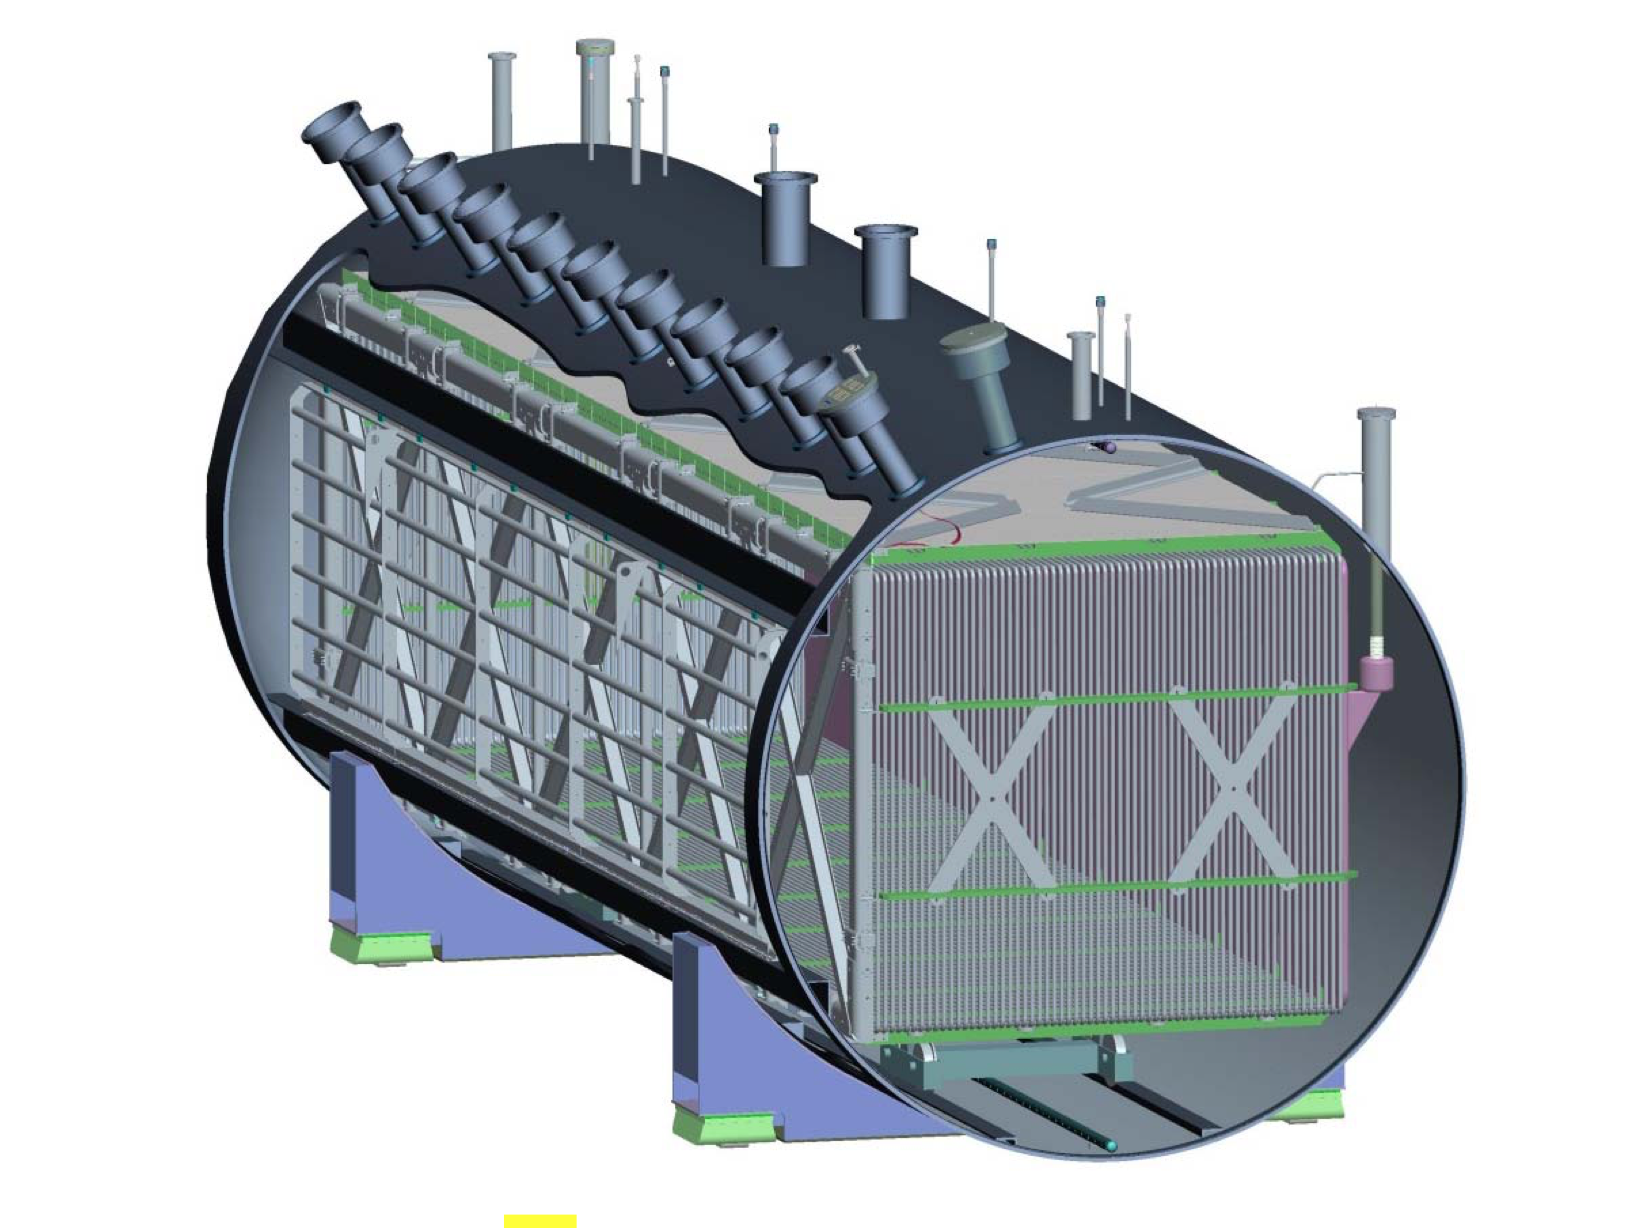
\includegraphics[scale=0.35]{Figures/uboone_cryo.png}
        \caption[MicroBooNE's LArTPC inside the cryostat]{{\textbf{MicroBooNE's LArTPC inside the cryostat}} \\ Schematic view of MicroBooNE's LArTPC inside of the cryostat vessel. The cryostat is the cylindric-like structure in the figure \cite{microboone_design}.}
        \label{uboone_cryo} 
    \end{center}
\end{figure}

\subsection{Light Collection System}

As mentioned in chapter \ref{Chapter:1}, the scintillation light produced by a charged particle crossing the LArTPC gives information about the event's start time. From the difference between the time that the electrons are collected in the collection plane and the start time of the event, plus the knowledge of the drift velocity of the electrons in the detector, we recover the third dimension of the track reconstruction. In MicroBooNE, the drift velocity of the electrons is $1.14$ m/ms. 

This is only possible because LAr produces plenty of scintillation light ($\approx 10^4 $) photons/MeV, and this light is produced and propagated in LAr almost instantaneously ($\approx$ ns). The scintillation light is produced in LAr by two mechanisms: self-trapped excitation luminescence and recombination luminescence. Figure \ref{lar_excimers} is a diagram demonstrating those two processes. When a charged particle passes through the liquid argon, it ionizes or excites it. In the first case, it will result in light being produced by self-trapped excitation luminescence, which will produce a singlet state in $65\  $ of the cases, and a triplet state in $35\%$ of the cases. In the excitation case, it will produce light by recombination luminescence, producing a singlet state in half of the cases and a triplet state in the other half. In all cases, the light signal is suppressed by impurities in the LAr. Either process produces light with a peak at the $128$ nm wavelength \cite{lar_excimers}.
 
\begin{figure}[h!]
    \begin{center}
        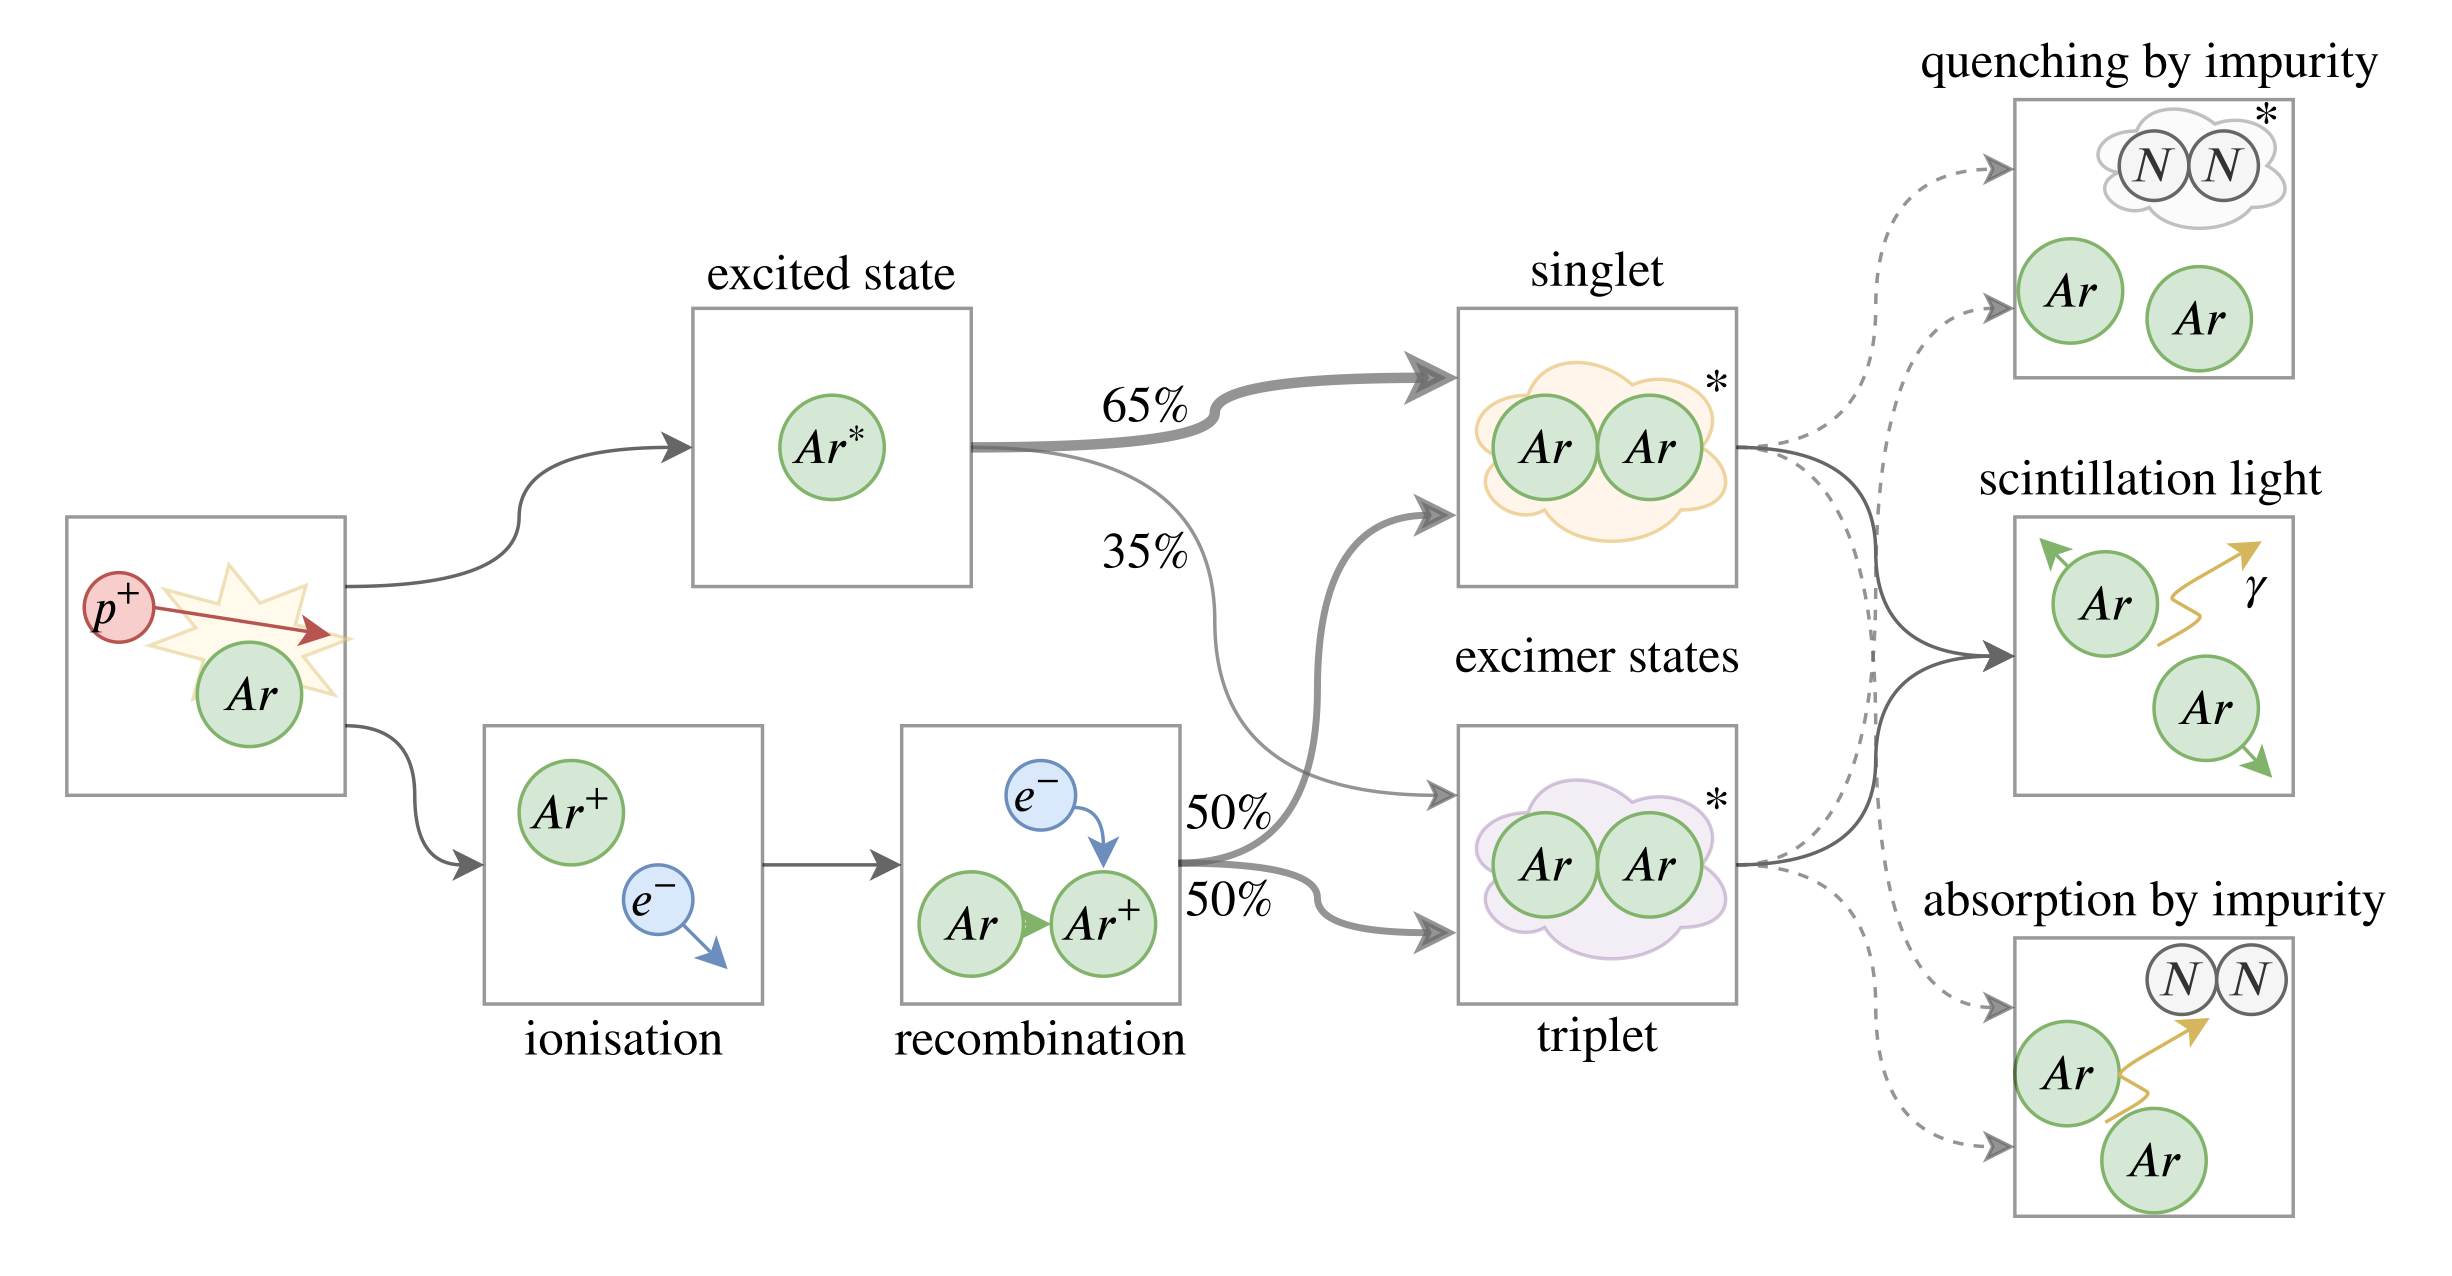
\includegraphics[scale=0.35]{Figures/lar_excimers.png}
        \caption[Scintillation light in liquid argon]{{\textbf{Scintillation light in liquid argon}} \\When a charge particle passes through the liquid argon, it ionizes or excites it. The light will be either produced by self-trapped excitationor by recombination. In all cases the light signal is supressed by impurities in the LAr \cite{lar_excimers}.}
        \label{lar_excimers} 
    \end{center}
\end{figure}
  
To detect this light signal, MicroBooNE has $32$ units of 8-inch Hamamatsu photomultiplier tubes (PMTs) arranged behind the APA. Each of them is covered with a plate coated in tetraphenyl butadiene (TPB) wavelength-shifter that absorbs the $128$ nm photons and re-emits them at $\approx425$ nm, which is compatible with the PMT's maximum quantum efficiency. A picture of a MicroBooNE PMT is in figure \ref{uboone_pmt}. Figure \ref{pmt_quantum_eff} shows the quantum efficiency of the PMTs used in MicroBooNE. 
  
\begin{figure}[h!]
    \begin{center}
        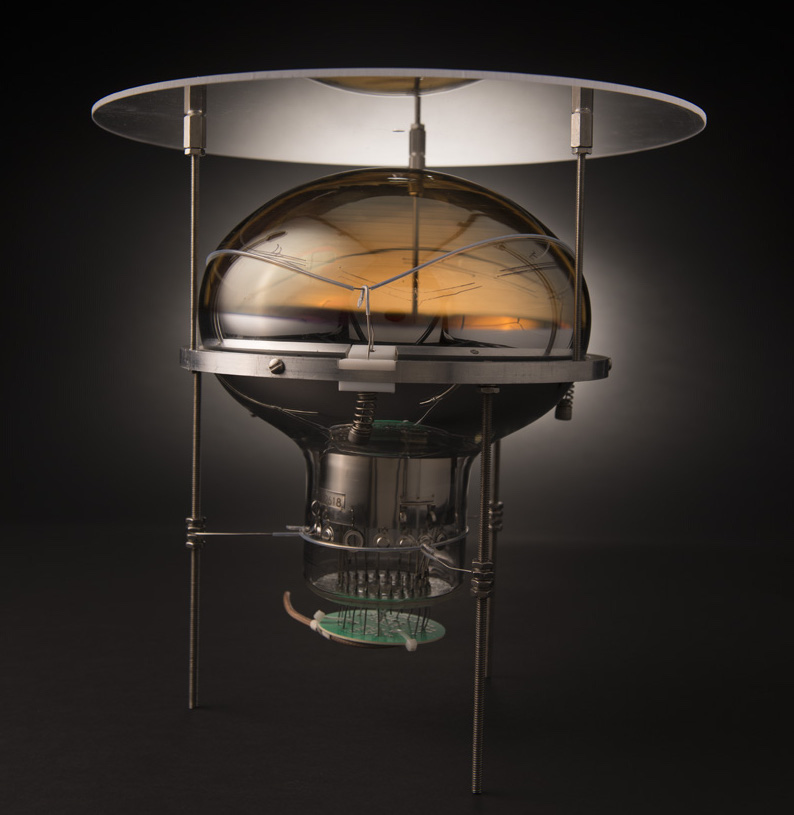
\includegraphics[scale=0.25]{Figures/microboone_pmt.jpeg}
        \caption[MicroBooNE's PMT]{{\textbf{MicroBooNE's PMT}} \\Picture of a $8$-inch Hamamatsu PMT used in MicroBooNE \cite{uboone_pmt}.}
        \label{uboone_pmt} 
    \end{center}
\end{figure}

\begin{figure}[h!]
    \begin{center}
        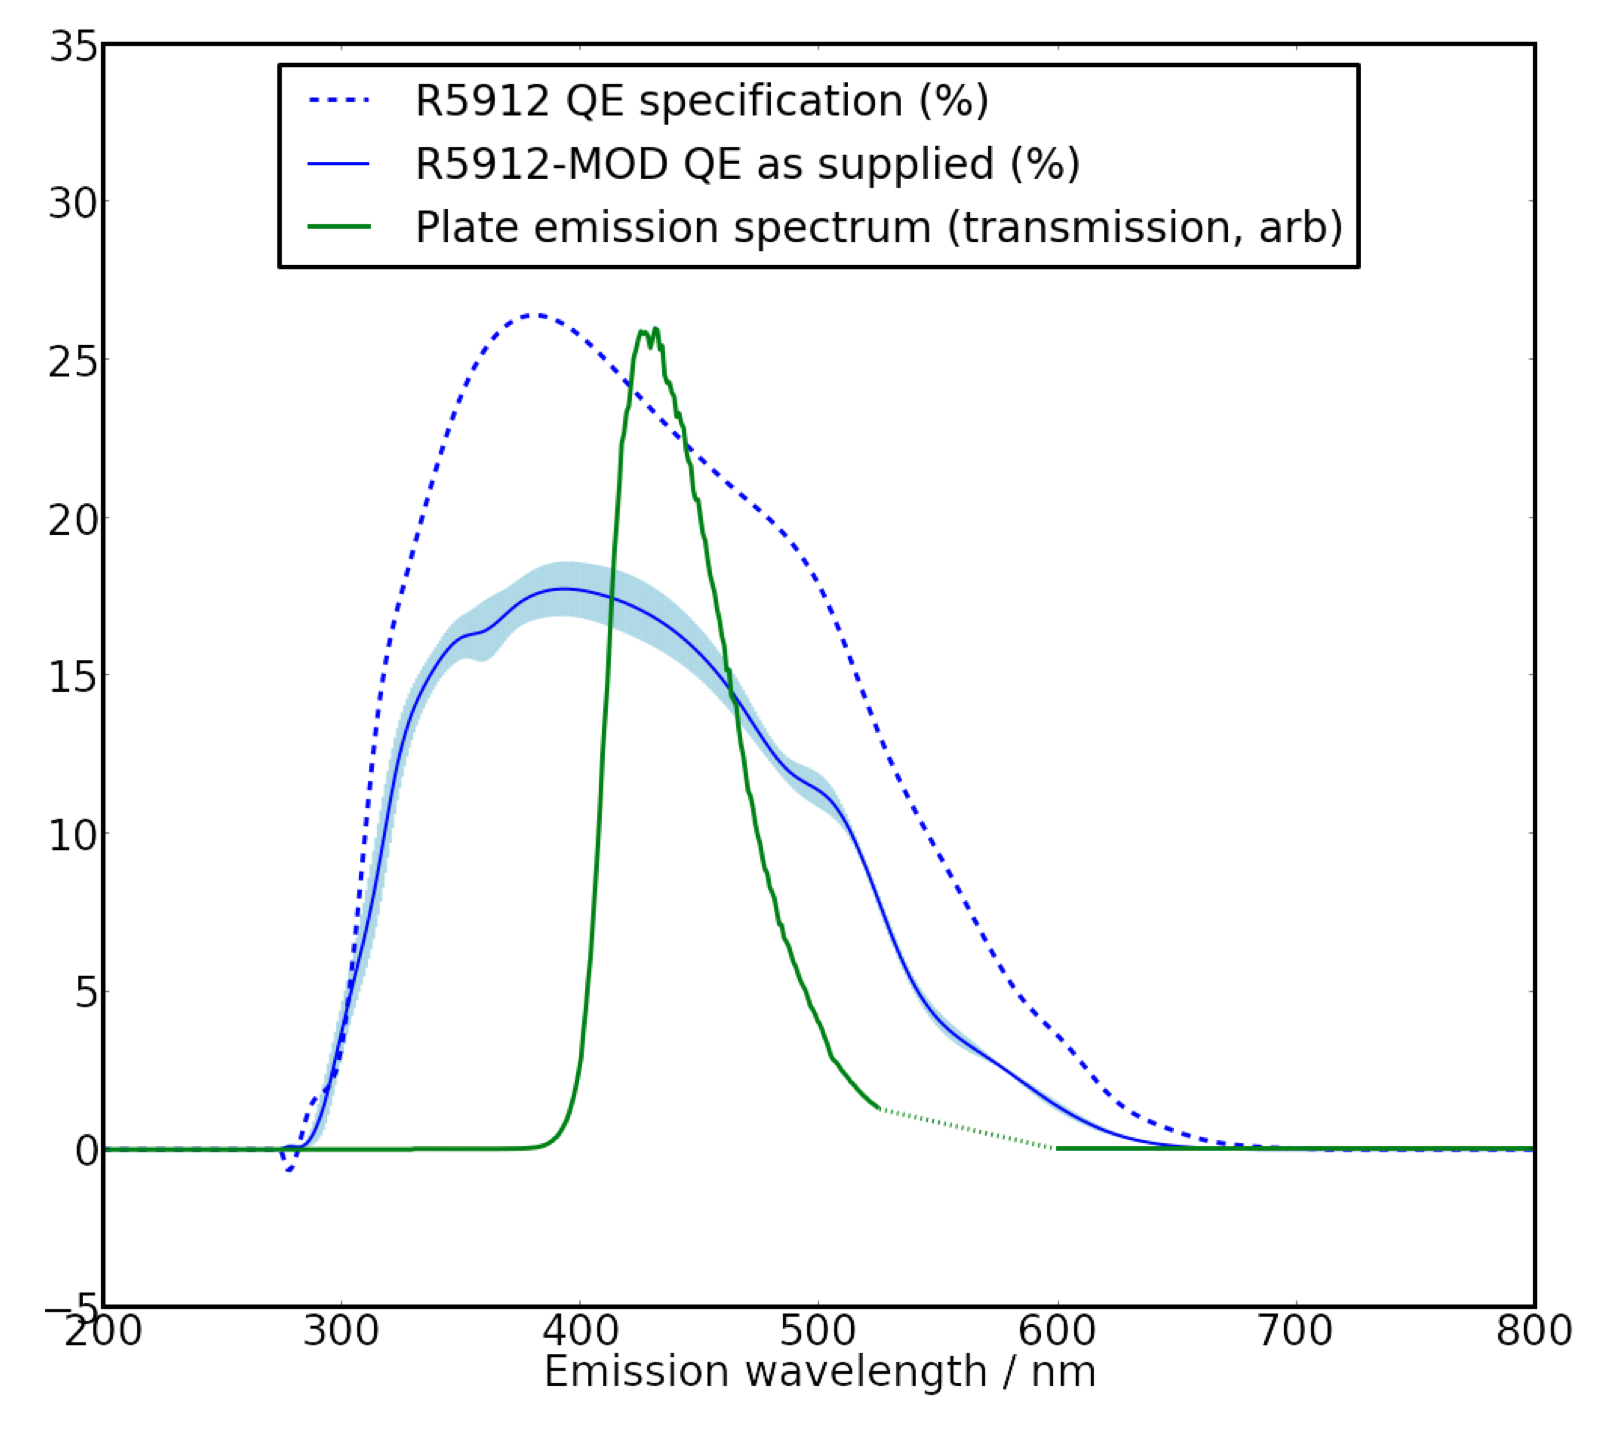
\includegraphics[scale=0.4]{Figures/quantum_eff.png}
        \caption[PMT's Quantum Efficiency]{{\textbf{PMT's Quantum Efficiency}} \\The specification for the non-platinum undercoated R5912 Hamamatsu PMT. The blue band shows the mean and standard deviation of the four quantum efficiency curves provided by Hamamatsu for the installed PMTs. Also shown is the measured emission spectra of the MicroBooNE wavelength-shifting coatings \cite{microboone_design}.}
        \label{pmt_quantum_eff} 
    \end{center}
\end{figure}
  

\section{Neutrino at the Main Injector (NuMI) Beamline}
  
To study neutrinos, Fermilab produces neutrinos through an accelerator chain that delivers two beams, the Booster Neutrino Beam and the Neutrino at the Main Injector beam. Both supply neutrinos to a variety of experiments. MicroBooNE's main beam is the BNB,  but it is also exposed to the NuMI beam. 
  
The accelerator chain (see full Fermilab's beam chain in figure \ref{accelerator_chain}) starts with an ion source machine with a molybdenum cathode installed inside of it and filled with hydrogen gas. The molybdenum's electrons are excited and then collected by the hydrogen atoms. The result is a H$^-$ gas. An ``extractor" attracts the negative atoms with a positive potential, pulling them through a hole with a width of a few mm. At the same time, a magnetic field guides them in the right direction to feed the beam into a radio-frequency quadrupole (RFQ). The RFQ receives the low-energy beam from the ion source at one end and ejects a $750$ keV \cite{RFQ_website} beam out of the other end, delivering it to a linear accelerator (LINAC). The LINAC is $150$ m long and is divided into two acceleration parts. The first is a drift tube that accelerates the beam up to $116$ MeV, and the second is a side-coupled cavity that accelerates the beam up to $401$ MeV \cite{LINAC_website}. Exiting the LINAC, the beam collides with a thin carbon sheet that removes electrons from the H$^-$, resulting in three beams: a $H^-$ beam, a $H^+$ beam, and a $H^0$ beam. Only the pure proton beam is selected. After these processes, the beam is suitable to be inserted into a circular $75$ m radius accelerator called the Booster, from which an $8$ GeV beam of protons is extracted that can be directed towards the Main Injector (MI), the BNB target, or to the Recycler \cite{booster_website}. For the NuMI beam, the protons from the Booster are directed towards a $3319.4$ m circumference synchrotron, called the Main Injector, that further accelerates the protons up to $120$ GeV. Those protons are then directed towards a graphite target, where they collide, producing the NuMI beam.
  
\begin{figure}[h!]
	\begin{center}
		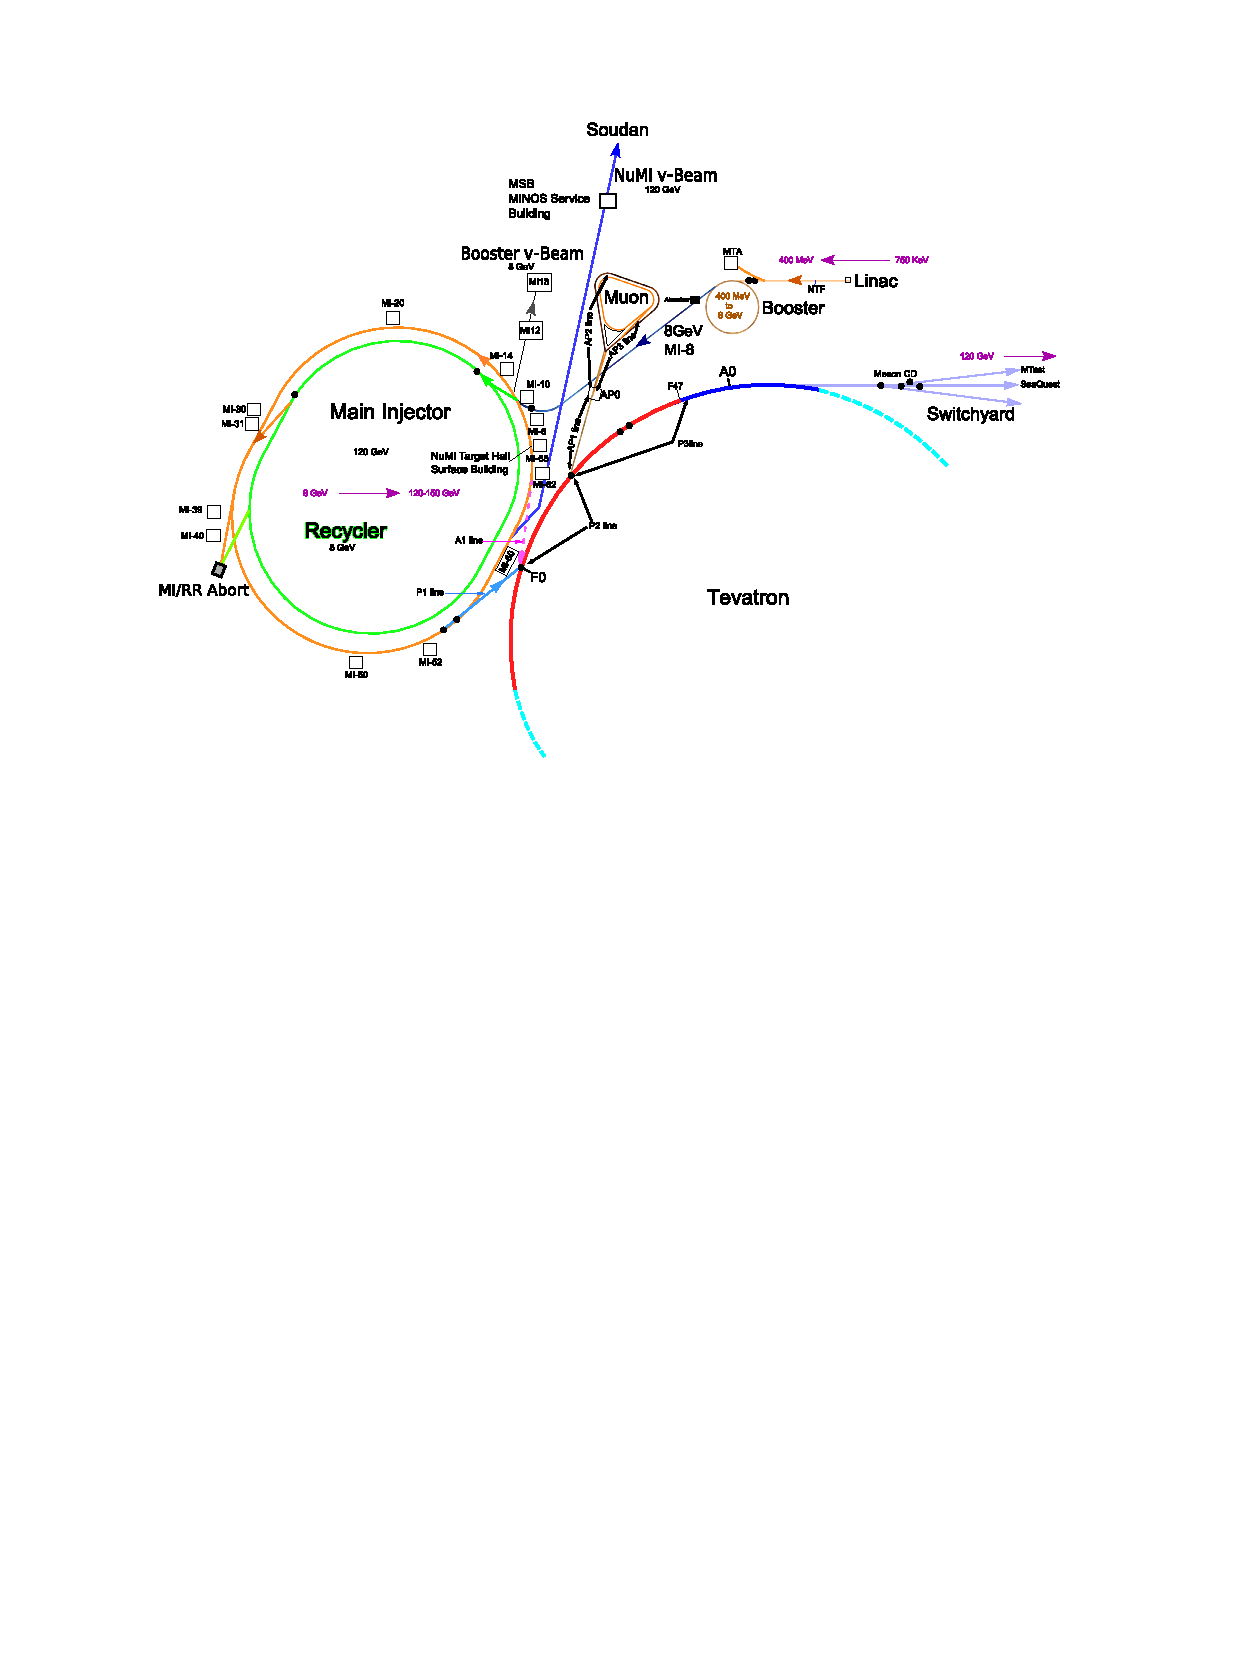
\includegraphics[scale=0.8]{Figures/acceleratorChain.pdf}
		\caption[Full Fermilab's beam chain]{ {\textbf{Full Fermilab's beam chain}} \\The image shows the Fermilab beam chain map, from the RFQ/LINAC to the main injector, BNB, or to the recycler \cite{paper_numibeamline}.}
		\label{accelerator_chain}	
	\end{center}
\end{figure}
  
In the NuMI beam, when the $120$ GeV protons impinge upon a graphite target, they produce mesons, including charged pions and kaons. These mesons are focused by magnetic horns and directed to the $675$ m long decay pipe, where they decay into muons and muon-neutrinos, as shown in the schematic view of the beamline in figure \ref{fig:numi}. After the decay pipe, an absorber blocks the remaining hadrons and muons in the beamline, allowing only the neutrinos to pass through. 
  
\begin{figure}[h!]
    \centering
    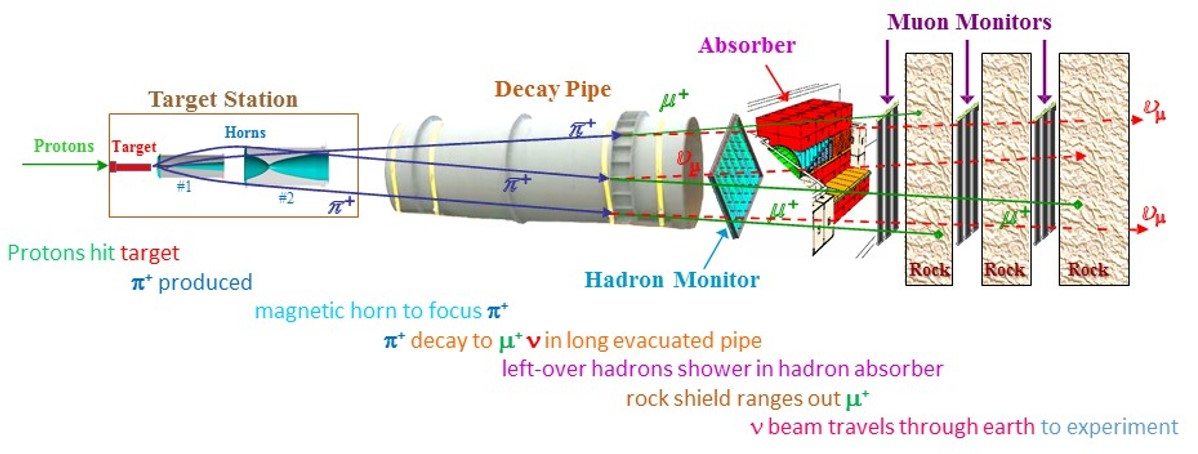
\includegraphics[width=140mm]{Figures/numi.jpg}
    \caption[NuMI layout]{{\textbf{NuMI layout}} \\Layout of the NuMI beamline \cite{numi}.}
    \label{fig:numi}
\end{figure}
  
By changing the polarity of the magnetic horns, we can select the sign of the charged mesons. By having a positive horn current, we select positive particles. We call it the Forward Horn Current (FHC) mode, or Neutrino Mode. By having a negative horn current, we select negative particles. We call it the Reverse Horn Current (RHC) mode, or Antineutrino Mode. In figure \ref{beam_mode_uboone} you can find a plot of the number of Protons on Target (POT) delivered in each run of MicroBooNE and in which mode the beam was selected. The NuMI beam delivers neutrinos in windows of $9.6 \mu$s. During MicroBooNE's operation time we collected a total of $2.3\times 10^{21}$ POT, $1.0\times10^{21}$ in Neutrino Mode and $1.3\times10^{21}$ in Antineutrino Mode
 
\begin{figure}[h!]
    \centering
    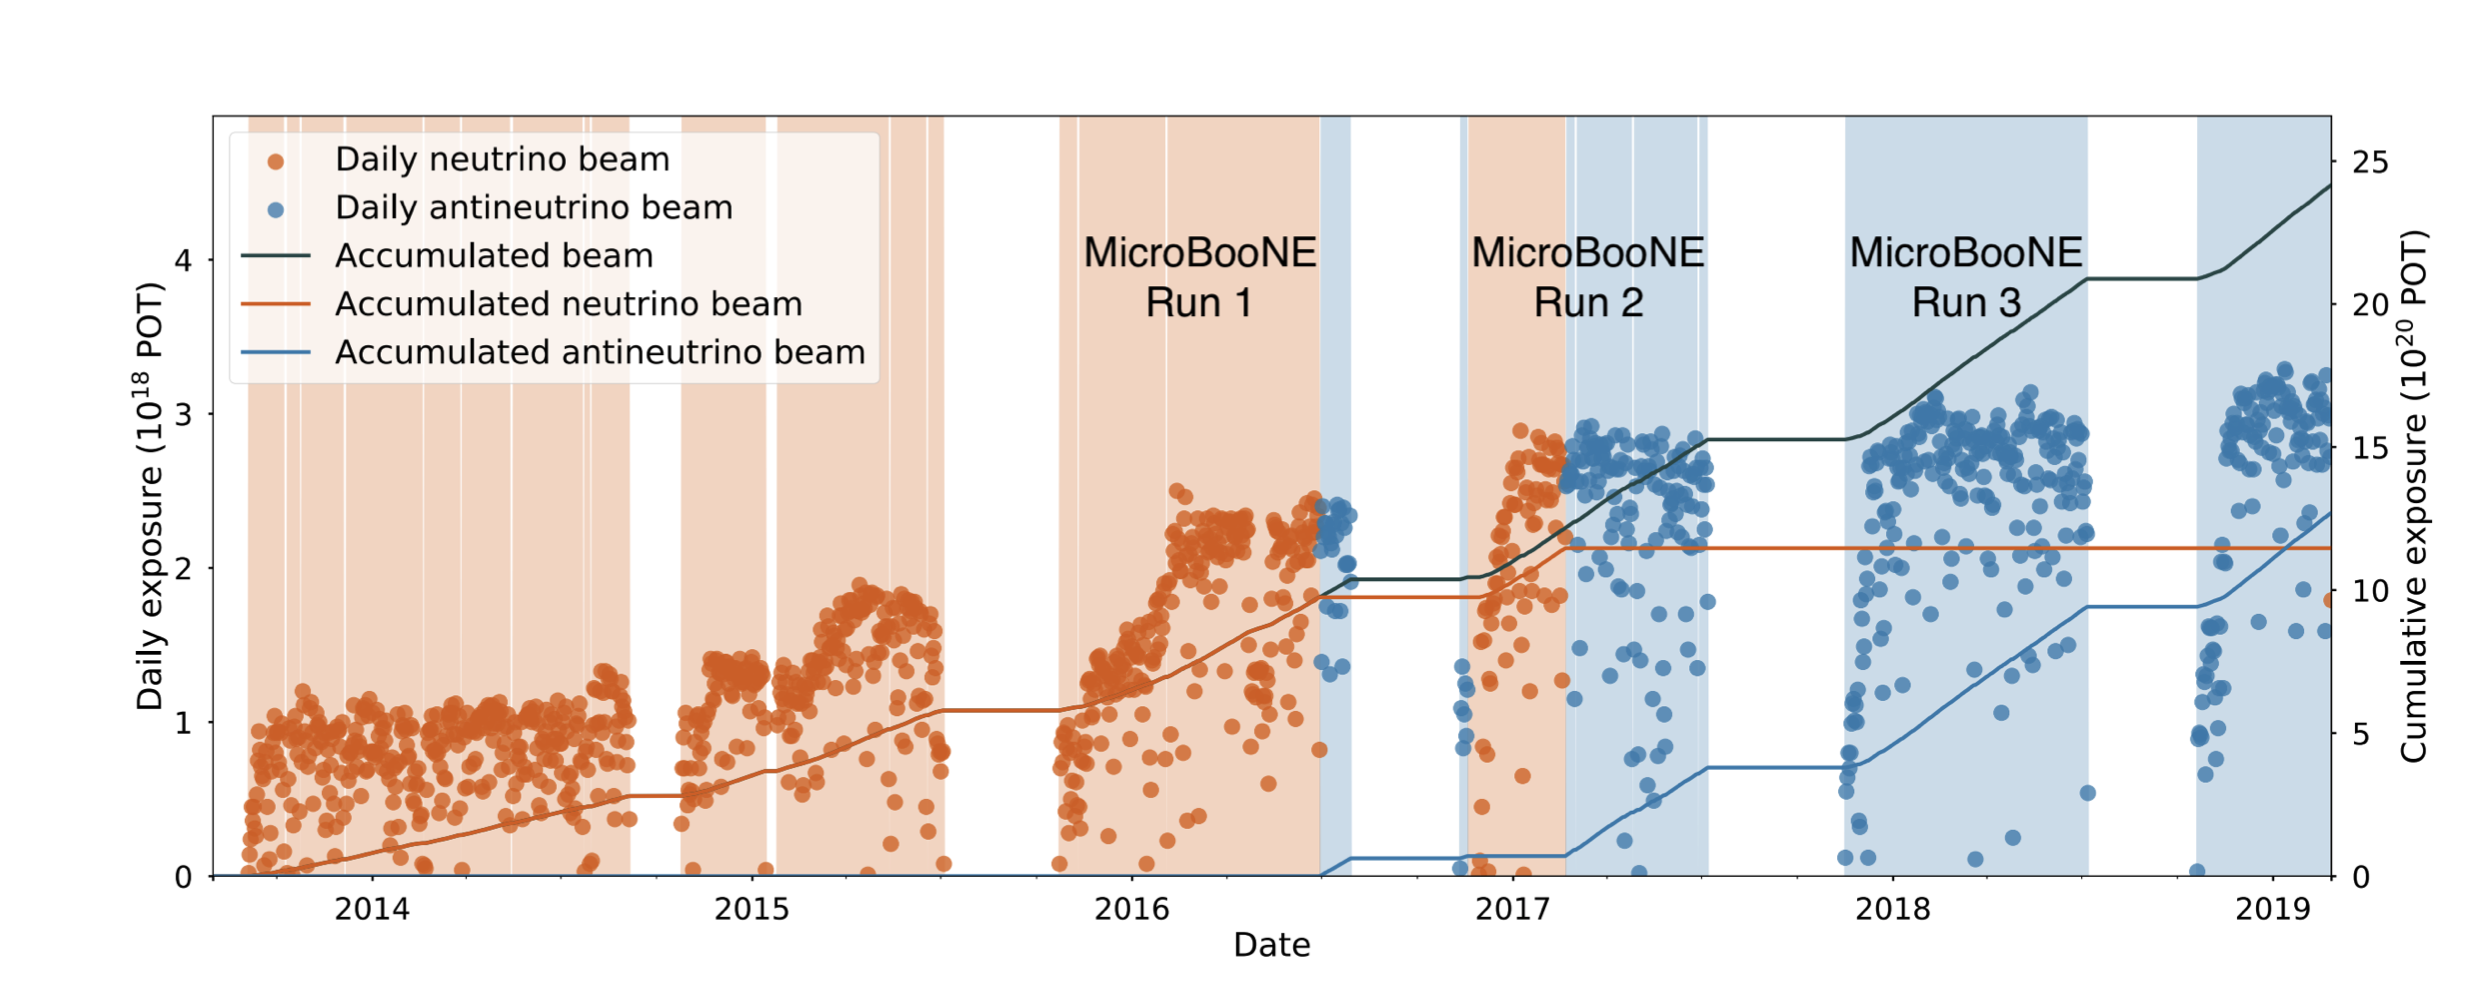
\includegraphics[width=150mm]{Figures/beam_mode_uboone.png}
    \caption[The total cumulative POT delivered by the NuMI beamline to MicroBooNE]{{\textbf{The total cumulative POT delivered by the NuMI beamline to MicroBooNE}}\\The cumulative POT from NuMI delievered to MicroBrooNE. In the orange regions the horn polarity was in Neutrino Mode. In the blue regions the horn polarity was in Antineutrino Mode. The white regions refer to periods in which the accelerator complex was shut down \cite{krish_phd}.}
    \label{beam_mode_uboone}
\end{figure}
  
\section{MicroBooNE's Readout and Trigger Systems}
  
As a surface detector, MicroBooNE's PMTs and TPC receive particle activity all the time, and recording all this data would be impossible. Additionally, only $2-3\%$ of the pulses of protons sent to the target (called ``spills") to produce the neutrinos in the NuMI beam will create a neutrino interaction in MicroBooNE. We use a trigger system to decide what data is recorded.
The trigger system starts with a signal from Fermilab's accelerator complex informing us they sent a new spill. This signal is our hardware (HW) trigger. The HW trigger gives a start to what we call the``beamgate window", in which we start the readout without any light intensity requirement (also known as ``unbiased"), which lasts $23.4$ $\mu $s. This happens $1.6$ ms into the TPC readout frame. The NuMI beam spill time window goes from $5.64- 15.44$ $\mu$s into the beamgate window. The complete readout cycle takes 3 TPC readout frames, which takes a total of $4.8$ ms.
The data collected is then passed to a buffer where a software will decide what will be permanently recorded on tape. This is our software (SW) trigger. To be recorded, the SW trigger requires the data to have at least $9.5$ PE of scintillation light in a time window of $4.69- 16.41$ $\mu$s from the beginning of the beamgate window. To account for some decline in the PMTs, during Run 3, the light requirement was updated to $5.75$ PE \cite{numi_redmine}. 
Around $14\%$ of all HW triggers pass the SW trigger conditions. 

Please see the diagram in figure \ref{trig} for a visual of the readout and trigger structure.

\begin{figure}[h!]
    \centering
    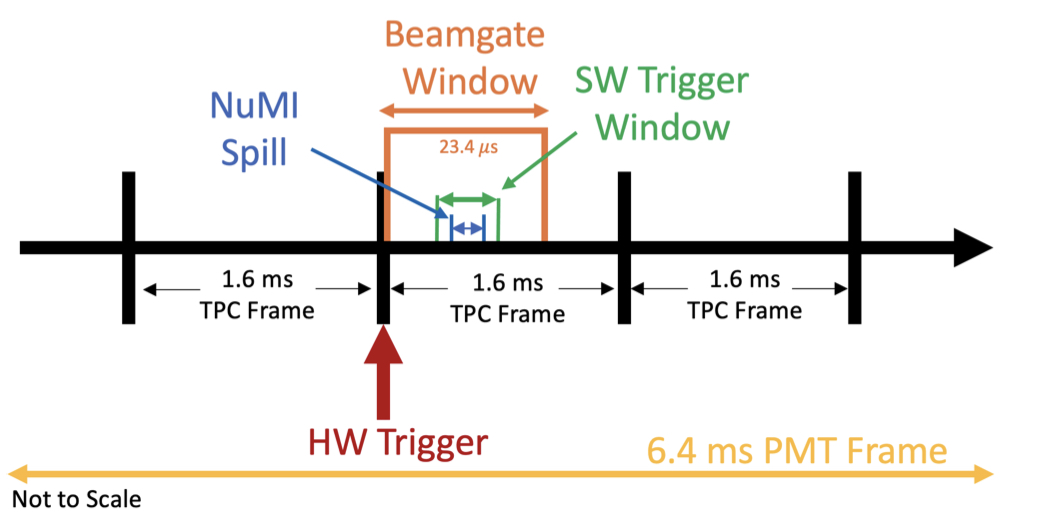
\includegraphics[width=150mm]{Figures/numi_trigger.jpg}
    \caption[MicroBooNE's NuMI readout and trigger]{\textbf{MicroBooNE's NuMI readout and trigger}\\Structure of MicroBooNE's NuMI readout and trigger \cite{krish_phd}.}
    \label{trig}
\end{figure}

From the data collected, MicroBooNE produces three data streams:
\begin{itemize}
 \item NuMI: For this stream, the data has to pass both the hardware and software triggers described above. It is also referred to as ``beam-on" data. 
 \item EXT NuMI: This is some data that passes the light requirements of the software trigger but is outside the beamgate window. The light is produced by cosmic rays, and this data is essential for us to understand the background of the neutrino analysis. It is also called ``beam-off" data. 
 \item EXT unbiased: This is data that is not in the beamgate window but with no additional requirements. Data from this stream is used to make our simulated events more realistic, as we overlay them with the simulated neutrino interactions. The procedure we use for that is documented in \cite{afro_phd}. 
\end{itemize}

MicroBooNE has a similar data stream, readout, and trigger systems for the BNB beam but with its own time windows. The beamgate window for the BNB and NuMI beams do not overlap. 